\documentclass[a4paper]{article}
\usepackage[utf8]{inputenc}
\usepackage[spanish, es-tabla, es-noshorthands]{babel}
\usepackage[table,xcdraw]{xcolor}
\usepackage[a4paper, footnotesep = 1cm, width=20cm, top=2.5cm, height=25cm, textwidth=18cm, textheight=25cm]{geometry}
%\geometry{showframe}

\usepackage{tikz}
\usepackage{amsmath}
\usepackage{amsfonts}
\usepackage{amssymb}
\usepackage{float}
\usepackage{graphicx}
\usepackage{caption}
\usepackage{subcaption}
\usepackage{multicol}
\usepackage{multirow}
\setlength{\doublerulesep}{\arrayrulewidth}
\usepackage{booktabs}

\usepackage{hyperref}
\hypersetup{
    colorlinks=true,
    linkcolor=blue,
    filecolor=magenta,      
    urlcolor=blue,
    citecolor=blue,    
}

\newcommand{\quotes}[1]{``#1''}
\usepackage{array}
\newcolumntype{C}[1]{>{\centering\let\newline\\\arraybackslash\hspace{0pt}}m{#1}}
\usepackage[american]{circuitikz}
\usetikzlibrary{calc}
\usepackage{fancyhdr}
\usepackage{units} 

\graphicspath{{../Ejercicio-1/}{../Ejercicio-2/}{../Ejercicio-3/}{../Ejercicio-4/}}

\pagestyle{fancy}
\fancyhf{}
\lhead{22.01 Teoría de Circuitos}
\rhead{Mechoulam, Lambertucci, Rodriguez Turco, Londero, Galdeman}
\rfoot{\centering \thepage}
\begin{document}
	\subsection{PLL: Phase-locked loops}
	\subsubsection{Introducción}
	Los circuitos \textbf{PLL} fueron introducidos a en el año 1960. Sin embargo, su concepto ya había sido probado 30 años atrás pero las limitaciones tecnológicas de la época. Son utilizados en diversas aplicaciones en el área de RF. Se emplean para demodular FM y FSK, acondicionamiento de señales y síntesis de frecuencias. En este trabajo nos dedicaremos a analizar como utilizar un PLL para demodular una señal de FM y a sintetizar una señal cuya frecuencia sea múltiplo de otra. Además estudiaremos el comportamiento del circuito bajo diferentes condiciones.
	
	\subsubsection{Diagrama en bloques de un PLL}
	El PLL consiste de 3 bloques fundamentales:
	
	\begin{enumerate}
		\item  Comparador
		\item  Filtro pasa bajos (LPF)
		\item  VCO (voltage controlled oscilator) 
	\end{enumerate}
	
	\begin{figure}[H]
		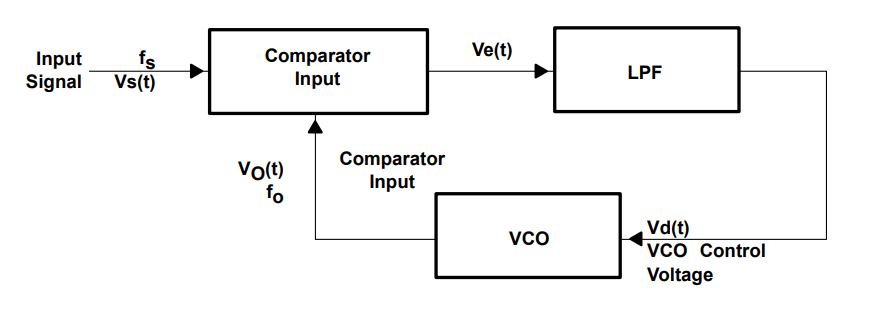
\includegraphics[width=\linewidth]{ImagenesVarias/PLLblockDiagram.PNG}
		\caption{Diagrama en bloques de un PLL}
	\end{figure}
El comparador emite una señal de error proporcional a la diferencia de frecuencia y fase con respecto a la señal de entrada. De no haber entrada (es decir tensión nula) el VCO operara a la frecuencia central ya configurada. La señal de error $V_e(t)$ es filtrada para asegurar que el VCO reciba una señal continua en su entrada. La configuración de retroalimentación busca minimizar la tensión de error. Para esto el VCO ajustara su frecuencia de operación. Por ejemplo, supongamos que la frecuencia central del VCO es $1Khz$ y nuestra entrada opera a $2Khz$. En este caso la señal de error proporcional a dicha diferencia forzara al VCO a aumentar su frecuencia de oscilación. Cuando nuestra frecuencia de entrada se aproxima a la frecuencia de central del VCO se dice que entra al \emph{Rango de captura o enganche}. Al entrar en esta zona y por efecto del circuito de realimentación, el VCO sincroniza su frecuencia de oscilación con aquella en la entrada del PLL.



\begin{figure}[H]
	\centering
	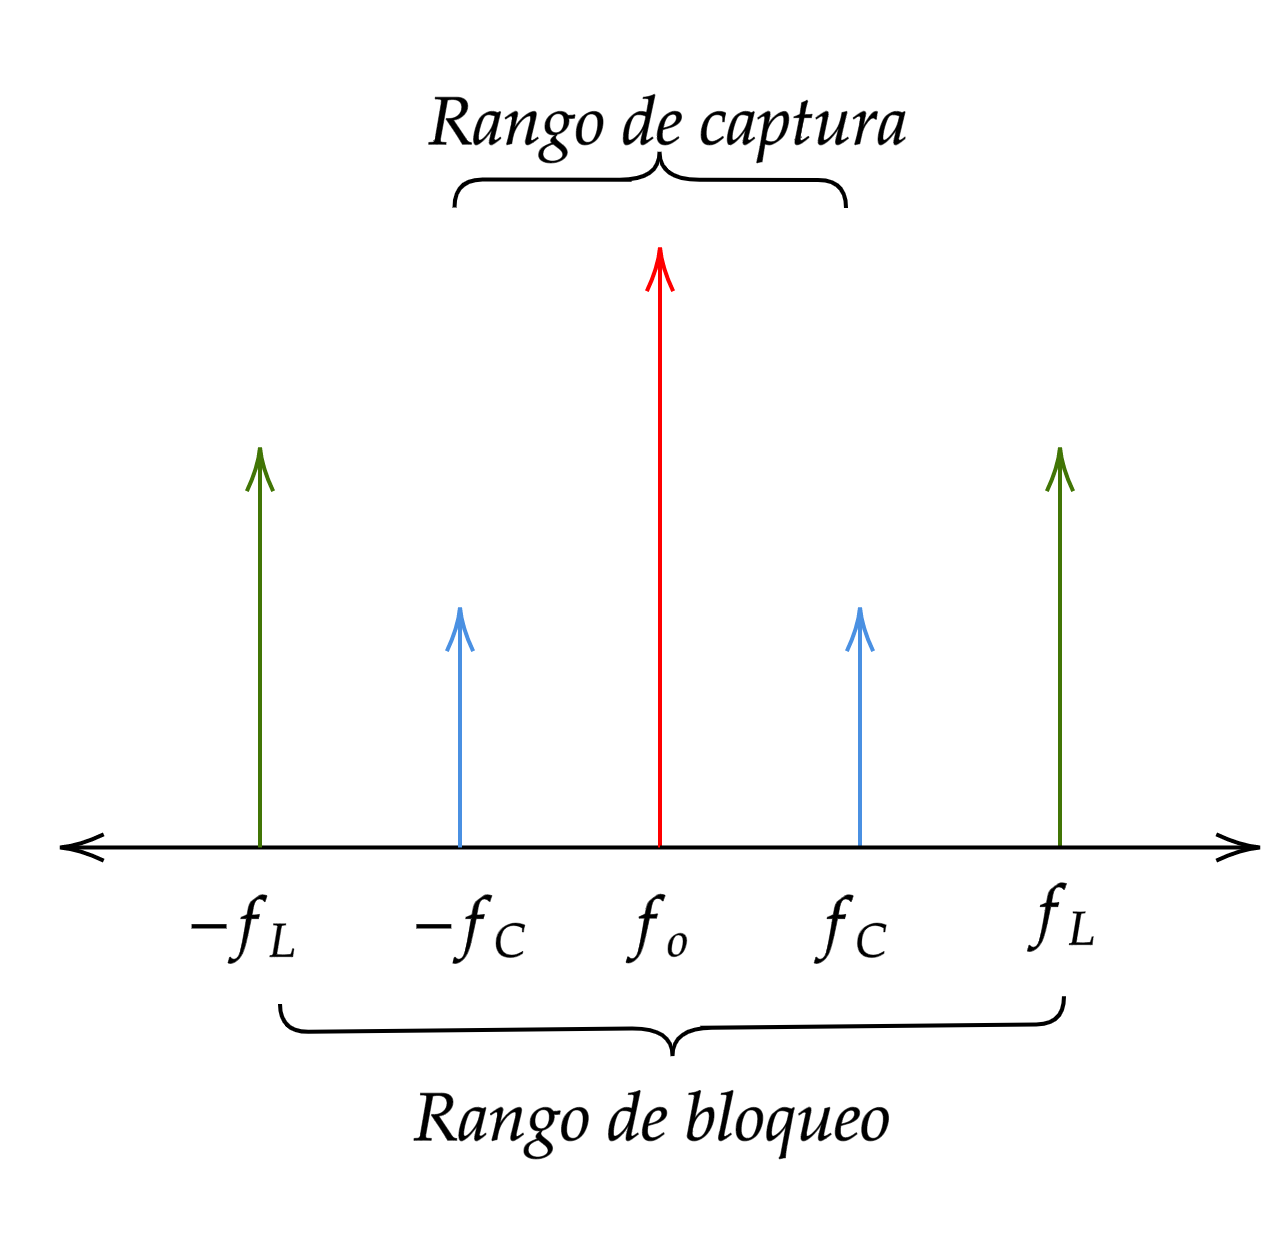
\includegraphics[scale=0.3]{ImagenesVarias/PLL_range2.png}
	\caption{Rango de bloque y enganche}
	\label{blockLockRange}
\end{figure}

Como podemos observar en la figura \ref{blockLockRange}. Existe la ya antes mencionada \textbf{zona de captura}. Una señal que se encuentre en este rango de frecuencias forzara al PLL a sincronizar la frecuencia de oscilación de su VCO interno con la frecuencia de la señal entrante. U na vez dentro de esta zona es posible utilizar el PLL dentro de la llamada \textbf{zona de bloqueo}. En esta zona el PLL mantendrá la frecuencia de oscilación sincronizada. Notemos que el rango de bloqueo es más grande que el rango de captura.

\subsubsection{Diseño y configuración}



\subsubsection{Síntesis de frecuencias}
Los circuitos PLL son utilizados para la síntesis de frecuencias. Para conseguirlo se recurre a colocar un divisor de frecuencia  la salida del VCO. Entonces el comparador de fase y frecuencia reconocerá que para igualar la frecuencia de entrada deberá forzar al VCO a aumentar la frecuencia de oscilación
\end{document}



%Notas
%

%https://sites.google.com/site/ccolonelec101/wentworth-institute-of-technology/electronic-design/phase-lock-loop